%% Widmung
\thispagestyle{empty}
\begin{center}
\vspace*{\fill}
%\it \ldots Widmung oder Motto \ldots
\vfill
\end{center}
\cleardoublepage


%% Motto
\thispagestyle{empty}
\begin{center}
\vspace*{\fill}
\begin{tabular}{c}
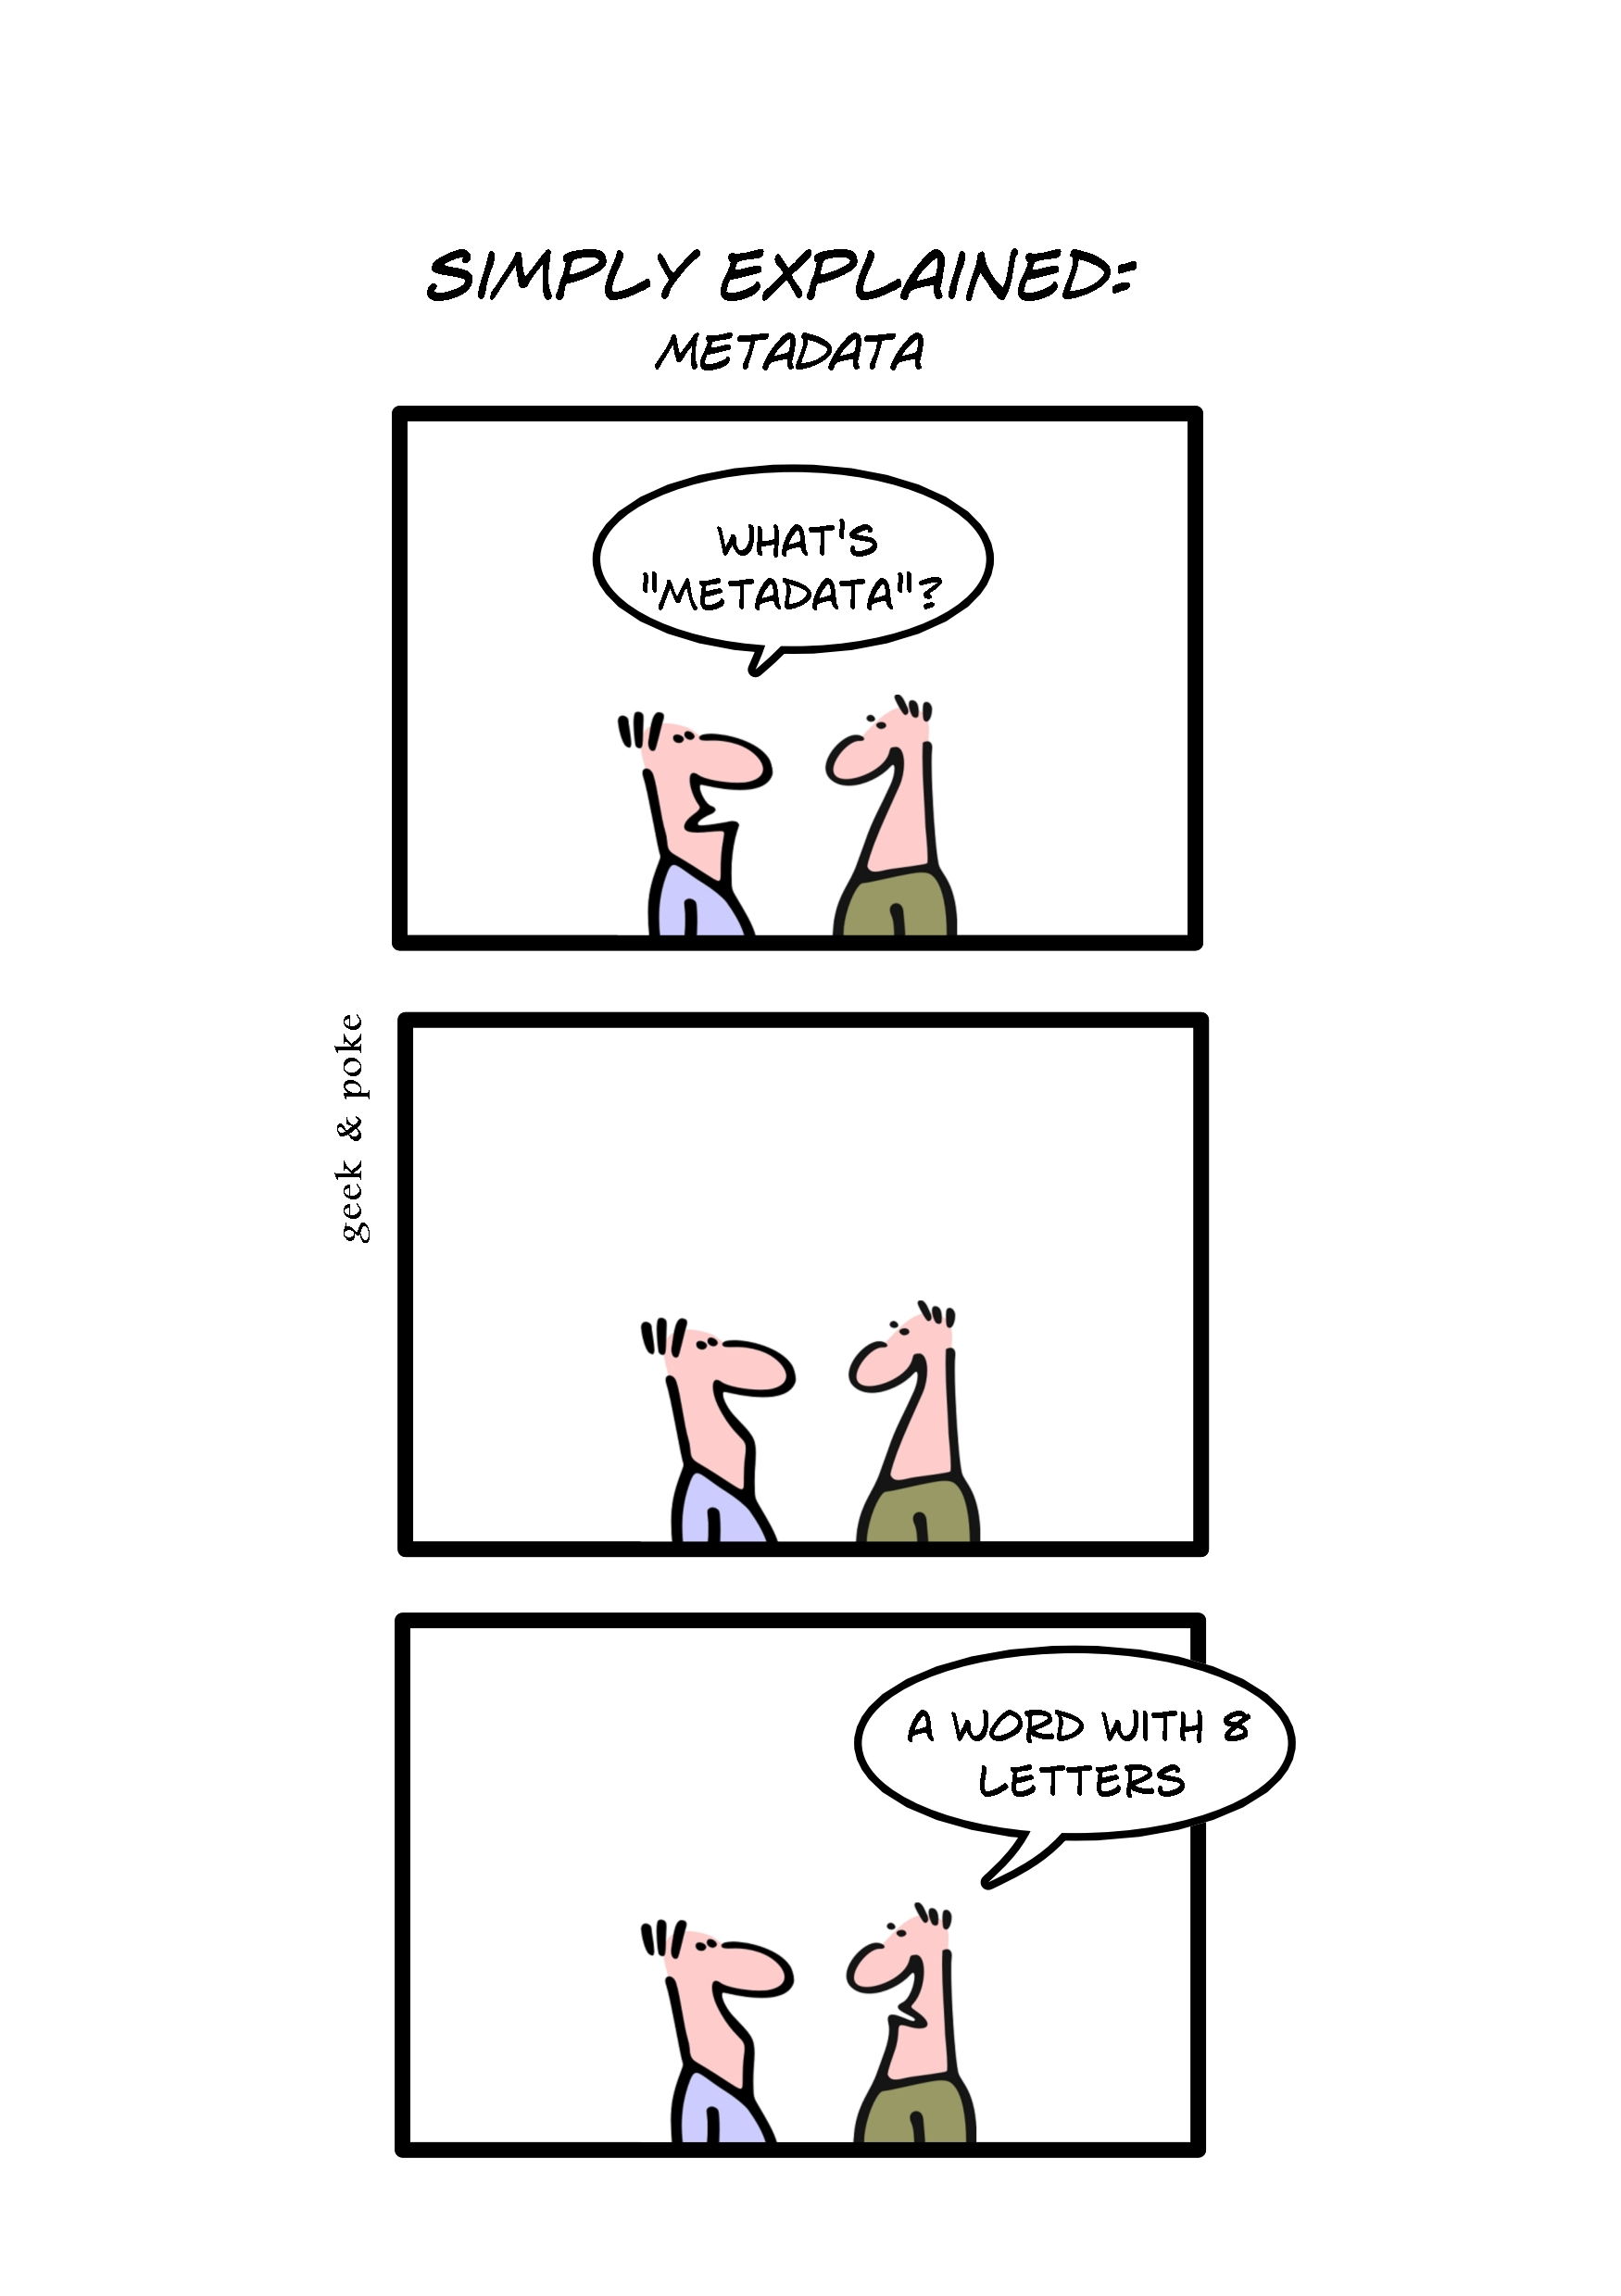
\includegraphics[width=12cm]{img/geekandpokemetadata.jpg} \\
CC-BY-SA by \textcite{Widder2010} \\
\end{tabular}
\vfill
\end{center}

\unnumberedsection{Abstract}
% English abstract, up to 2000 characters

Many methods, technologies, standards, and languages exist to structure and
describe data. The aim of this thesis is to find common features in these
methods to determine how data is actually structured and described. Existing
studies are limited to notions of data as recorded observations and facts, or
they require given structures to build on, such as the concept of a record or
the concept of a schema. These presumed concepts have been deconstructed in
this thesis from a semiotic point of view. This was done by analysing data as
signs, communicated in form of digital documents.  The study was conducted by a
phenomenological research method.  Conceptual properties of data structuring
and description were first collected and experienced critically. Examples of
such properties include encodings, identifiers, formats, schemas, and models.
The analysis resulted in six prototypes to categorize data methods by their
primary purpose. The study further revealed five basic paradigms that deeply
shape how data is structured and described in practice.  The third result
consists of a pattern language of data structuring.  The patterns show problems
and solutions which occur over and over again in data, independent from
particular technologies.  Twenty general patterns were identified and
described, each with its benefits, consequences, pitfalls, and relations to
other patterns. The results can help to better understand data and its actual
forms, both for consumption and creation of data. Particular domains of
application include data archaeology and data literacy.

% Data is not not measured or observed but created
% Intellectial analysis of data (not statistical pattern recognition)

\begin{otherlanguage}{ngerman}
\unnumberedsection{Zusammenfassung}

% See http://www.uq.edu.au/student-services/phdwriting/phlink08.html
% Eine Mustersprache zur Datenstrukturierung und -beschreibung

%\textit{Deutscher Text (bis zu 2000 Zeichen).}
% http://de.wikipedia.org/wiki/Ph%C3%A4nomenologie_%28Methodik%29
% http://wiki.zum.de/Ph%C3%A4nomenologische_Methode

% 1. Prototypensemantik
% 2. Paradigmen
% 3. Mustersprache

Diese Arbeit behandelt die Frage, wie Daten grundsätzlich strukturiert und
beschrieben sind. Im Gegensatz zu vorhandenen Auseinandersetzungen mit Daten im
Sinne von gespeicherten Beobachtungen oder Sachverhalten, werden Daten hierbei
semiotisch als Zeichen aufgefasst. Diese Zeichen werden in Form von digitalen
Dokumenten kommuniziert und sind mittels zahlreicher Standards, Formate,
Sprachen, Kodierungen, Schemata, Techniken etc. strukturiert und beschrieben.
Diese Vielfalt von Mitteln wird erstmals in ihrer Gesamtheit mit Hilfe der
phenomenologischen Forschungsmethode analysiert. Ziel ist es dabei, durch eine
genaue Erfahrung und Beschreibung von Mitteln zur Strukturierung und
Beschreibung von Daten zum allgemeinen Wesen der Datenstrukturierung und
-beschreibung vorzudringen. Die Ergebnisse dieser Arbeit bestehen aus drei
Teilen. Erstens ergeben sich sechs Prototypen, die die beschriebenen Mittel
nach ihrem Hauptanwendungszweck kategorisieren. Zweitens gibt es fünf
Paradigmen, die das Verständnis und die Anwendung von Mitteln zur
Strukturierung und Beschreibung von Daten grundlegend beeinflussen. Drittens
legt diese Arbeit eine Mustersprache der Datenstrukturierung vor. In zwanzig
Mustern werden typische Probleme und Lösungen dokumentiert, die bei der
Strukturierung und Beschreibung von Daten unabhängig von konkreten Techniken
immer wieder auftreten. Die Ergebnisse dieser Arbeit können dazu beitragen, das
Verständnis von Daten --- das heisst digitalen Dokumente und ihre Metadaten in
allen ihren Formen --- zu verbessern. Spezielle Anwendungsgebiete liegen unter
Anderem in den Bereichen Datenarchäologie und Daten-Literacy.

\end{otherlanguage}
\cleardoublepage

%% Inhaltsverzeichnisse
\tableofcontents

%% Die weiteren Verzeichnisse alle direkt hintereinander
\begingroup
\let\cleardoublepage\relax
\let\clearpage\relax
\makeatletter\renewcommand*{\float@listhead}[1]{\unnumberedsection{#1}}\makeatother
\listof{example}{List of Examples}
\listoffigures
\listoftables
\endgroup

